\documentclass[11pt, a4paper]{article}

% --- Essential Packages ---
\usepackage[utf8]{inputenc}    % Text encoding
\usepackage{graphicx}          % Required for inserting images
\usepackage{url}               % Required for robust URL handling
\usepackage{hyperref}          % Required for links and URLs
\usepackage{geometry}          % Adjust page margins
\geometry{margin=2.5cm}

% --- Document Information ---
\title{\textbf{Labwork 4 Report: Threads}}
\author{Lucien Elyas Bedrane \\ Student ID: 2640012}
\date{\today}

\begin{document}

\maketitle

% --- Section 1: Objective Breakdown ---
\section{Objectives \& Breakdown}
This lab is a continuation of labwork 3 where we improve our previous work in order to use 2D version of our Grayscale function.

% --- Section 2: Code Output Image ---
\section{Implementations \& Results}
To improve upon the code we made last time, I first started to work on the blockSize and gridSize so that they could be used for our 2D calculations.
\\For this, I implemented what was described in the course, i.e., a list of 2D tuples for blockSize and gridSize where for blockSize : (x,y) with x = y and for gridSize, I simply modified the labwork 3 function to use the height and width of the image. 
\\Lastly, I rounded up every result (both for the 1D and 2D verisons) to the upper integer to make sure that enough blocks are allocated so that every single data element has a corresponding thread to process it. This information was found on Nvidia CUDA Programming course (link available at the Sources and References section).
\\On the image below is a graph showcasing the different time required to process the image using the 1D and the 2D versions of Grayscale.
\\As the 2D version uses a (x,x) tuples for its block size, the blocks used are squared (i.e.: 32 blocks means $32^{2}$ = 1024 blocks) :
 
\begin{figure}[h!]
    \centering
    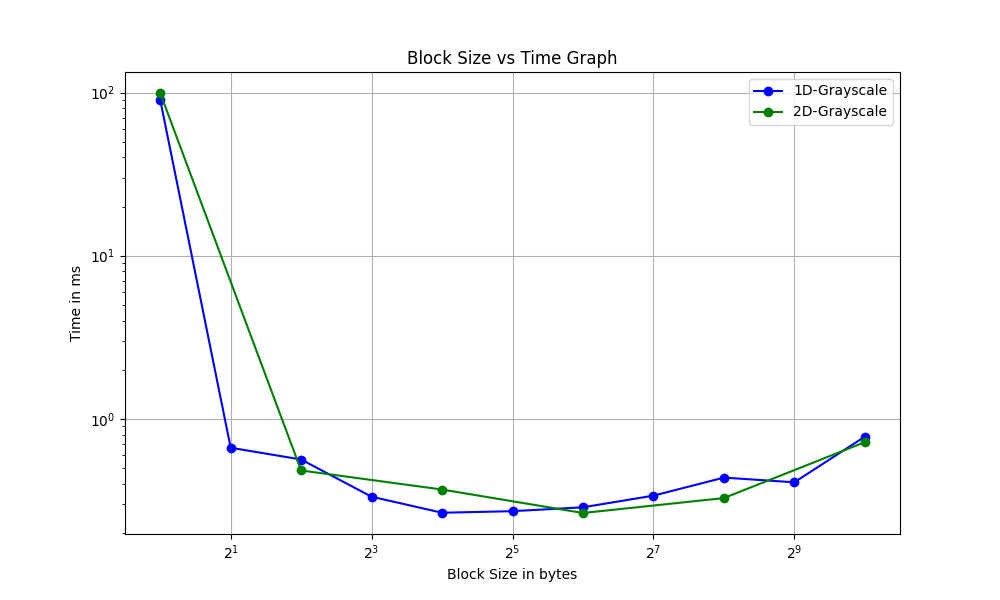
\includegraphics[width=0.8\textwidth]{plots/BlockSize_vs_Time_Graph} 
    \caption{Block size vs Time graph.}
    \label{fig:graph}
\end{figure}

As we can see in this graph, both functions have almost similar graphs. The higher the block size, the better the 2D version seems to be (except for a block size value of $2^{10}$ where we reach the limit of our GPU).
\\Using a bigger image may show a different result as the 2D version will handle in a better way the access to memory compared to the 1D version.

% --- Section 3: Sources ---
\section{Sources \& References}
The following resources and documentation were used to complete this work:

\begin{itemize}
    \item Thread and Memory Model by Tran Giang Son for M2 at ICT\\
    \item Nvidia CUDA Programming Guide \\
    \url{https://docs.nvidia.com/cuda/cuda-programming-guide/02-basics/intro-to-cuda-cpp.html#bounds-checking}
\end{itemize}

\end{document}
